\chapter[Revisão de Literatura]{Revisão de Literatura}

%\addcontentsline{toc}{chapter}{Revisão de Literatura}
% ----------------------------------------------------------

\section{Busca de caminhos}

\subsection{O Algoritmo A*}

O algorítimo A* é um dos mais populares soluções no ramo de busca de caminhos, o algoritmo garante achar o menor caminho entre dois pontos \cite{PEHart}, porem gera uma grande arvore de busca nos processos, consumindo muito tempo e memoria, é comum haver modificações no algorítimo para explorar uma arvore de busca menor, diminuindo o tempo para achar um caminho sacrificando a garantia de se encontrar o melhor caminho no final. \cite{Botea}.

O algoritmo A* em sua forma tradicional, utiliza a formula heurística f(n) = g(n) + h(n), onde g(n) é o custo para chegar ao nó n, e h(n) é o custo estimado para atingir o nó de destino a partir do nó n. Este cálculo pode ser realizado pela distância Manhattan. Para cada iteração sobre os vizinhos do nó atual é calculado o f(n) e adicionado em uma lista de nós abertos (A). Depois é verificado na lista o menor valor de f(n), este é removido, adicionado a lista de nos fechados (F) e a partir desse ponto, ele se torna o nó atual, quando o nó atual é o mesmo nó de destino o algorítimo retorna o caminho encontrado, assim podemos encontrar a solução ideal .

Podemos aplicar o algoritmo A* em um Grafo direcionado ponderado facilmente (Figura 1)



\begin{minipage}{\linewidth}
    \makebox[\linewidth]{
        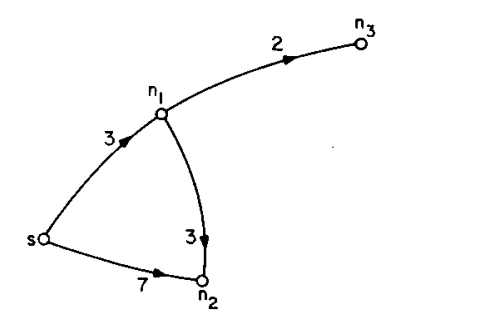
\includegraphics[keepaspectratio=true,scale=0.5]{ibagens/figura1.png}}
    \captionof{figure}{Grafo para busca \cite{PEHart}}
\end{minipage}


\begin{description}
    \item[Figura 1] Consiste em um nó inicial s e mais três outros nós (n1,n2,n3). As arestas contem a direção e o custo do trajeto. Se partirmos do algorítimo A* para produzir um subgrafo do melhor caminho, partindo de s podemos ir para n1 e n2, os valores de g(n1) e g(n2) são respectivamente 3 e 7. Supondo que A* expanda n1, sucedido por n2 e n3, nesse ponto g(n3)=3+2=5,o valor de g(n2) é diminuído pois um caminho de menor custo foi encontrado  3+3=6, o valor de g(n1) continua sendo 3. 
    
\end{description}

A heurística fornece uma expansão considerável dos nós, que são mantidos na memoria durante todo o processamento. (Figura 2)




\begin{minipage}{\linewidth}
    \makebox[\linewidth]{
        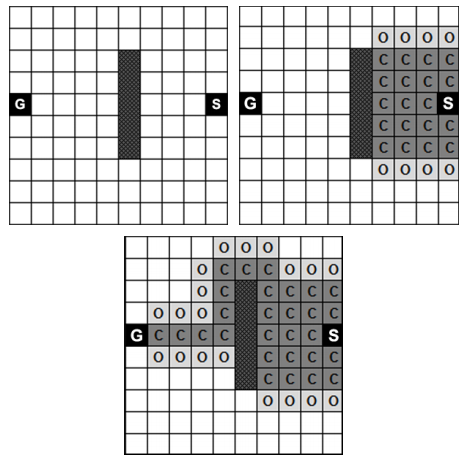
\includegraphics[keepaspectratio=true,scale=0.5]{ibagens/figura2.png}}
    \captionof{figure}{Exemplo de A* \cite{Ulysses} }
\end{minipage}

\subsection{Aplicações}
Aplicações para os algoritmos de busca podem ser diversos, como por exemplo, em um simulador de carro corrida \cite{JungTing}. Utilizando o algoritmo do A* com duas modificações para encontrar o melhor caminho enquanto evita os obstáculos entre o ponto de inicio e o ponto de destino. 
A primeira modificação consiste em utilizar o Teorema de Triângulos de Pytagoras, onde primeira calcula a distancia entre dois pontos(1 e 2), verifica se existe algum obstaculo dentre eles, se existir, utiliza o terceiro ponto para calcular a Hipotenusa e verifica se existe obstaculo entre a hipotenusa, se não existir, remove o ponto 2 e começa a considerar o caminho do ponto 1 para o ponto 3. A segunda modificação consiste em somente ir para frente, isso significa, procura somente os pontos a frente do carro, direita, esquerda e frente, simulando um controle de carro.
O projeto utiliza 3 pistas reais de corrida da Formula 1, Peru, Itália e Hungria, sendo cada pista, uma imagem de escala 1280x782 pixels retiradas do site oficial da Formula 1. O Carro é implementado em Microsoft XNA Game Studio, plataforma usada para desenvolver jogos para Windows Phone, Xbox e Windows. As Imagens das pistas são modificadas para serem mapas de detecção de colisão, a pista é pintada de preto, indicando onde o carro pode andar e o resto pintado de branco indicando os o carro não pode andar. O carro tem o tamanho de 18x12 pixels e uma movimentação de 2 pixels por segundo. Como o XNA trabalha com uma taxa de quadros de 60 quadros por segundo, o carro se movimenta a 120 pixels por segundo.
Os resultados da primeira modificação conseguiu economizar ciclos de CPU, reduzindo o numero de pontos indicadores da pista em 97\%. A segunda modificação tem a vantagem de obter o tempo de volta mais curto, por que reduz o numero de nós do algoritmo A* de 4 para 3 nós]. A desvantagem é que o carro pode balançar em curvas acentuadas. Em geral, as modificações garantiram uma melhoria em performance, economizando o numero de ciclos de CPU.

\section{Algorítimos genéticos}

\section{Algoritmos de busca paralelo}

\section{Algorítimos genéticos para busca de caminhos}
Buscando melhorar a eficiência dos algoritmos de busca, foram criadas formas hibridas, levando os algoritmos genéticos analisarem todo o percusso,ajudando o algoritmo de busca em momentos que a próxima ação é incerta.

Utilizando o algoritmo de busca BFS (\textit{Best First Search}), foi desenvolvido o modelo PPGA (\textit{Patterned based Pathfinding with Genetic Algorithm}). O modelo utiliza algoritmos genéticos como um modulo para calcular os sub caminhos ao longo do processo de busca, cada vez que o modulo é chamado, herda informações da chamada anterior, tendo um ganha considerado de desempenho. O modulo é chamado, quando nenhum dos valores dados pelo BFS são melhores que o valor atual. Os resultados da analise do PPGA foram bons, por encontrar boas soluções em um curto período de tempo, mostrando ser muito bom para mapas onde o percurso segue um padrão, mas perdendo para o BFS para mapas mistos ou que não seguem o mesmo padrão ao longo o percurso, considerando o modelo como promissor, indicando que mudanças nos parâmetros do algoritmo genéticos, pode melhorar o desempenho dos testes \cite{Ulysses}.
O modelo GAMMA(\textit{Genetic Algoritmo Manufactured Maneuvering Algorithm}), consiste em uma modificação do A* de forma que o caminho total é separado em caminhos mais curto. O algoritmo prepara o primeiro caminho e calcula o caminho mais curto entre eles, a posição final do resultado é usada como inicial para o próximo calculo, com isso, permitindo que o modelo GAMMA procure caminhos em tempo real por que se o caminho for alterado a sua leitura é parcial do caminho completo.\cite{Ryan}


\begin{minipage}{\linewidth}
	\makebox[\linewidth]{
		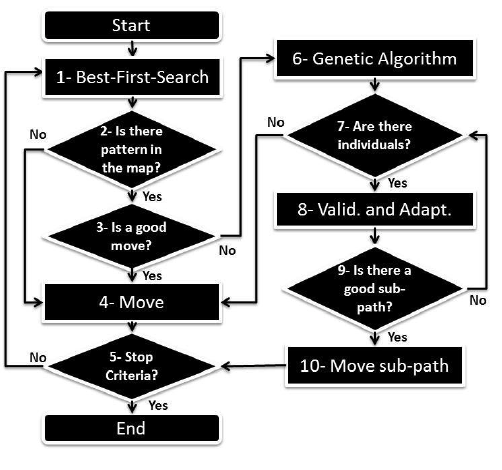
\includegraphics[keepaspectratio=true,scale=0.5]{ibagens/Fluxograma.png}}
	\captionof{figure}{Fluxograma do Modelo \cite{Ulysses} }
\end{minipage}

Utilizando o algoritmo de busca A*, foi desenvolvido o modelo

\section{Algorítimos genéticos paralelos ou distribuídos para busca de caminhos}

Foi demonstrado que algoritmos genéticos paralelos são eficientes para a resolução de problemas de busca de caminho, tal como o clássico problema do caixeiro viajante, que consiste em dado um numero finito de cidades com seus custos de viagem entre elas, deve-se encontrar o caminho mais curto para viajar entre todas as cidades e voltar ao ponto inicial. O problema pode ser representado pelo modelo de um grafo direcionado ponderado, aplicando a mesma ideia, o problema seria encontrar o caminho de menor custo para percorrer todos os nós, de maneira análoga, as cidades seriam os nós e a distancia entre elas, o peso das arestas \cite{Jason}\cite{Alaoui}\cite{Heinz}.

Os algoritmos genéticos exigem apenas o valor dado por uma função objetivo como parâmetro e mesmo sobre espaços de busca grandes, tem uma convergência rápida. Por causa do processo associado, agrega uma visão mais global do espaço de busca na prática de otimização e possuem uma fácil paralelizar por causa da independência dos seus processos. Em comparação com as técnicas de busca mais comuns,que requerem informações derivadas, continuidade do espaço de busca ou conhecimento completo da função objetiva.\cite{Vilson}.

A solução para este tipo de problema pode requer uma quantidade grande de processamento. Uma boa solução seria dividir o processamento do problema em pequenas partes e distribuir cada parte para um processador a parte, trabalhando de forma distribuída ou paralela. Vários modelos para essa finalidade foram propostos.

Um modelo interessante para paralelização seria o de mestre-escravo, onde o mestre fica responsável na manutenção da população e execução dos operadores genéticos. A avaliação dos melhores indivíduos é distribuída para os demais escravos, O mestre envia um indivíduo a cada um dos escravos subjacentes. Cada escravo realiza a interpretação do problema, aplica a função de cálculo para a escolha dos melhores indivíduos e envia seus resultados ao mestre, que executa seleção dos indivíduos e a geração da nova população, repetindo o processo como um todo. Essa estrutura teve implicação satisfatória para a automação de design de circuitos eletrônicos. \cite{Jason}

Outra forma de trabalhar com o modelo de mestre escravo, seria definir que cada um dos nós escravos subjacentes fica responsável por sua própria população. O nó central mestre, cria as populações iniciais e as distribui para os nós escravos. Cada nó escravo processa a evolução da população por um determinado número de gerações e então a submete ao mestre. O mestre então seleciona os melhores indivíduos dentre todas as populações dos nós escravos e os distribui novamente. Em cada nó escravo, os novos indivíduos distribuídos pelo mestre são inseridos na população corrente e o processo de evolução recomeça. A migração entre os escravos, que é controlado pelo nó mestre, implementa o mecanismo que regula a velocidade da convergência e oferece os meios de escape dos mínimos locais. Entretanto a migração das populações dos nós escravos para o mestre e vice versa pode impor um certo grau de sobre carga, dependente do meio de comunicação entre os nós. Esse modelo obteve sucesso no mapeamento de tarefas em maquinas paralelas. \cite{Alaoui}

Podemos partir do ponto que cada indivíduo é o responsável por encontrar e reproduzir com um parceiro em sua vizinhança. O controle de seleção e reprodução se espalha pela população e o algoritmo deixa de ser centralizado em um mestre, com isso, diminui o grau de sincronização e facilita a paralelização. O processo do algoritmo é definir uma representação genética para o problema e criar a estrutura de vizinhança e sua população inicial. Cada indivíduo faz uma busca em sua vizinhança e seleciona um parceiro para a reprodução. Uma geração descendente é criada com o operador genético resultante. \cite{Heinz}

Podemos observar alguns problemas nos modelos apresentados \cite{Vilson}, no modelo de \cite{Jason} existe problema em explorar o paralelismo no calculo de verificação dos indivíduos não explorando para a reprodução e mutação. No modelo de \cite{Heinz}, tem a possibilidade de utilizar vários métodos de busca de indivíduos da mesma população, sendo úteis em casos que a eficiência dos métodos de busca se mostram dependentes da instancia do problema. O modelo \cite{Alaoui}, por todos os escravos devem enviar para o nó mestre, demanda uma grande capacidade de processamento no nó mestre, e proporciona a divisão das populações em pequenas ou de médio porte.

 \cite{Vilson} desenvolveu seu próprio modelo, utilizando o modelo de \cite{Alaoui} como inspiração. O modelo segue o conceito mestre-escravo, o mestre crias as populações e distribui a cada uma delas, os conjuntos de genes e parâmetros iniciais. O mestre é utilizado para a troca de indivíduos entre as populações, mantendo um indivíduo de cada população até serem substituídos por um melhor e envia esses indivíduos para as populações que não seja a sua de origem. As populações são independentes, gerando seus indivíduos iniciais com base nos genes enviados pelo mestre, aplicando seus próprios operadores de evolução e a população que determina os parceiros dos indivíduos.